\documentclass[12pt,slidestop,handout]{beamer}
\usepackage[utf8]{inputenc}
\usepackage{german}
\usepackage{graphicx}
\beamertemplatenavigationsymbolsempty
\usetheme{Boadilla}
\usecolortheme{whale}
\setbeamertemplate{itemize items}[default]
\setbeamertemplate{enumerate items}[default]
\defbeamertemplate*{footline}{my infolines theme} {
\leavevmode
\hbox{
\begin{beamercolorbox}[wd=.333333\paperwidth,ht=2.25ex,dp=1ex,center]{author in head/foot}
\usebeamerfont{author in head/foot}\insertshortauthor
\end{beamercolorbox}
\begin{beamercolorbox}[wd=.333333\paperwidth,ht=2.25ex,dp=1ex,center]{title in head/foot}
\usebeamerfont{title in head/foot}\insertshorttitle
\end{beamercolorbox}
\begin{beamercolorbox}[wd=.309\paperwidth,ht=2.25ex,dp=1ex,center]{date in head/foot}
\usebeamerfont{date in head/foot}\insertshortdate{}\hspace*{2em}
\insertframenumber{} / \inserttotalframenumber\hspace*{2ex}
\end{beamercolorbox}}
\vskip0pt
}
\newcounter{FrameCounter}
\newcommand{\nextframe}[0]{\stepcounter{FrameCounter}}
\newcommand{\framecount}[1]{\frametitle{\arabic{FrameCounter}. {#1}}}
\newcommand{\fitem}{\vfill\item}
\newcommand{\TikZ}{Ti\textit{k}Z}

\title{FSML++ + Testing}
\author{Carsten Hartenfels \and Benjamin Haßel}
\date{2014-01-30}

\begin{document}
\begin{frame}
	\titlepage
\end{frame}

\begin{frame}
	\frametitle{Contents}
	\pause
	\begin{enumerate}[<+->]
		\fitem What
		\fitem Where
		\fitem How
	\end{enumerate}\vfill
\end{frame}

\nextframe
\begin{frame}
	\framecount{What}\pause
	\begin{itemize}[<+->]
	\fitem Identity Testing
	\begin{center}
		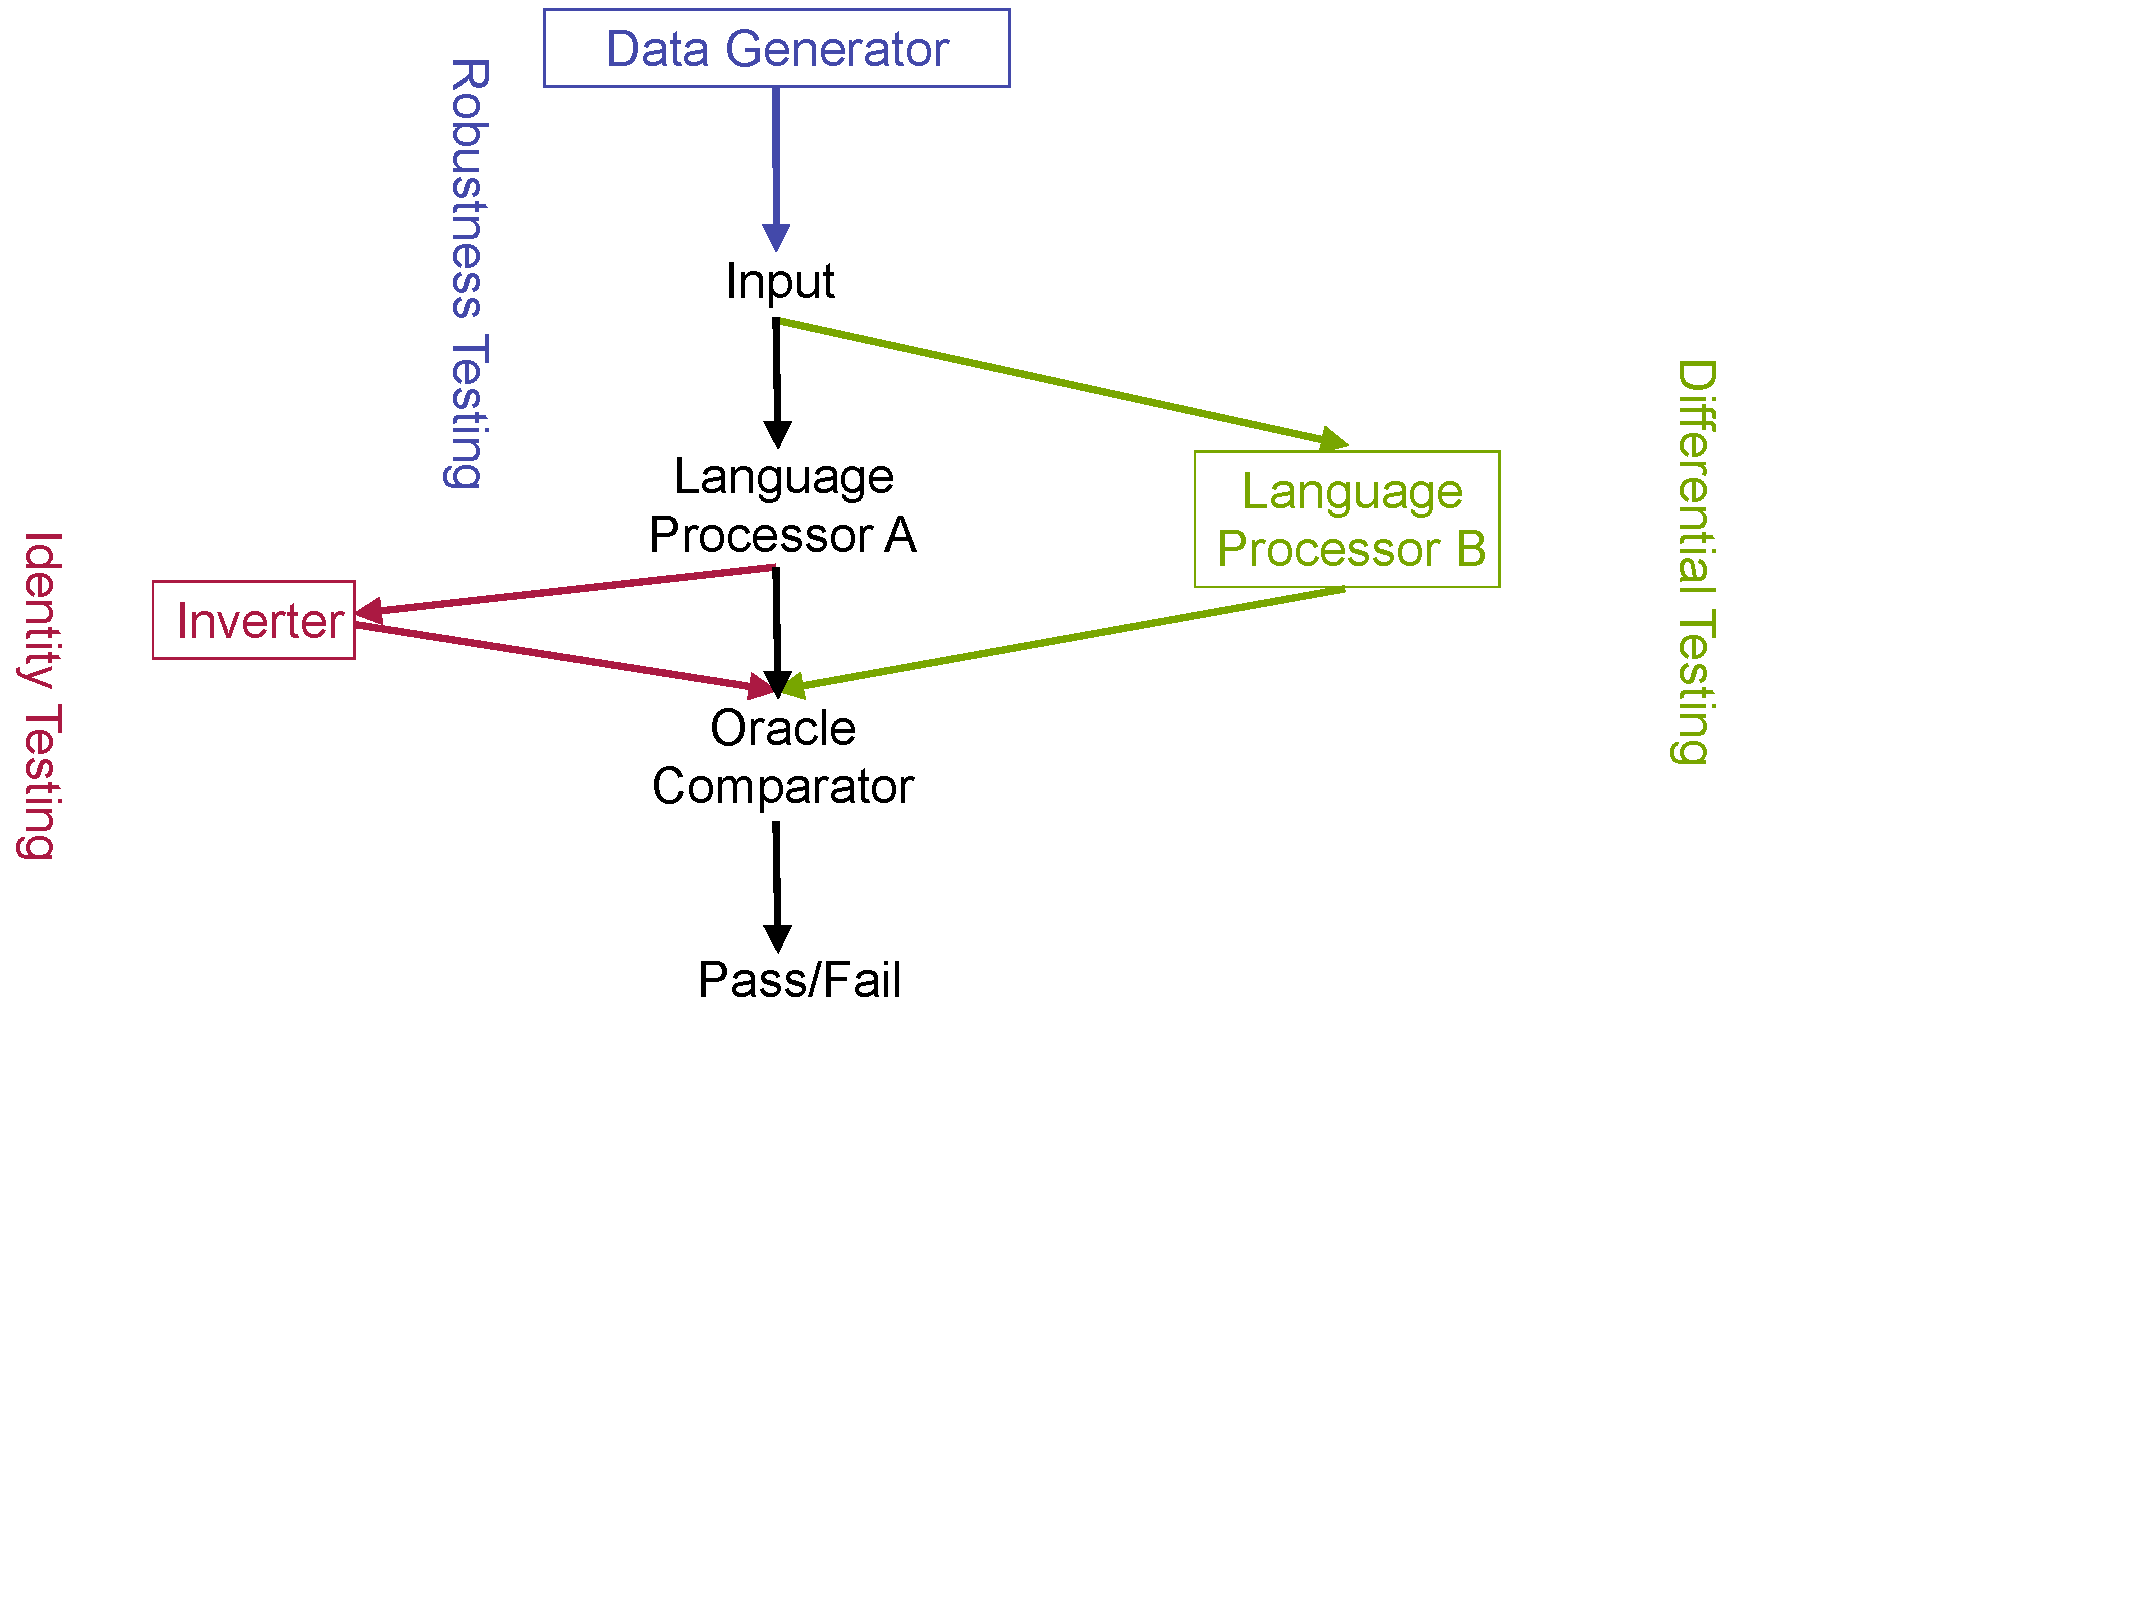
\includegraphics[scale=0.25]{res2/PageFromTesting.pdf}
	\end{center}
	\end{itemize}
\end{frame}

\nextframe
\begin{frame}
	\framecount{Where}\pause
	\begin{itemize}[<+->]
		\fitem Code Changes:
		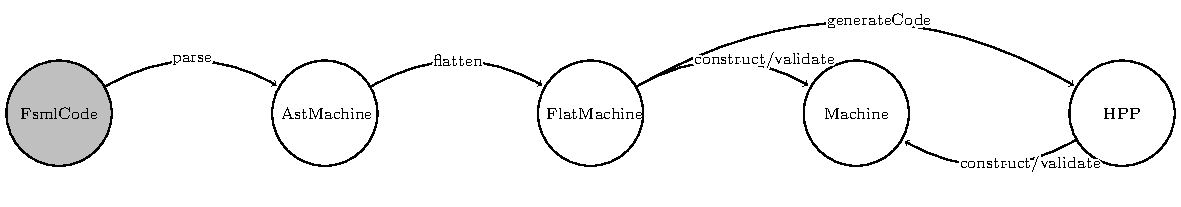
\includegraphics[scale=0.5]{res2/StructOld.pdf}\\
		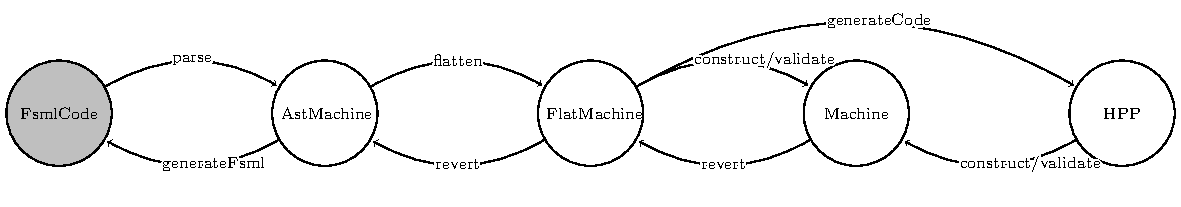
\includegraphics[scale=0.5]{res2/StructNew.pdf}
	\end{itemize}
\end{frame}

\nextframe
\begin{frame}
	\framecount{How}\pause
	\begin{itemize}[<+->]
	\fitem Testing environment undecided, but there oughta be one
	\begin{center}
		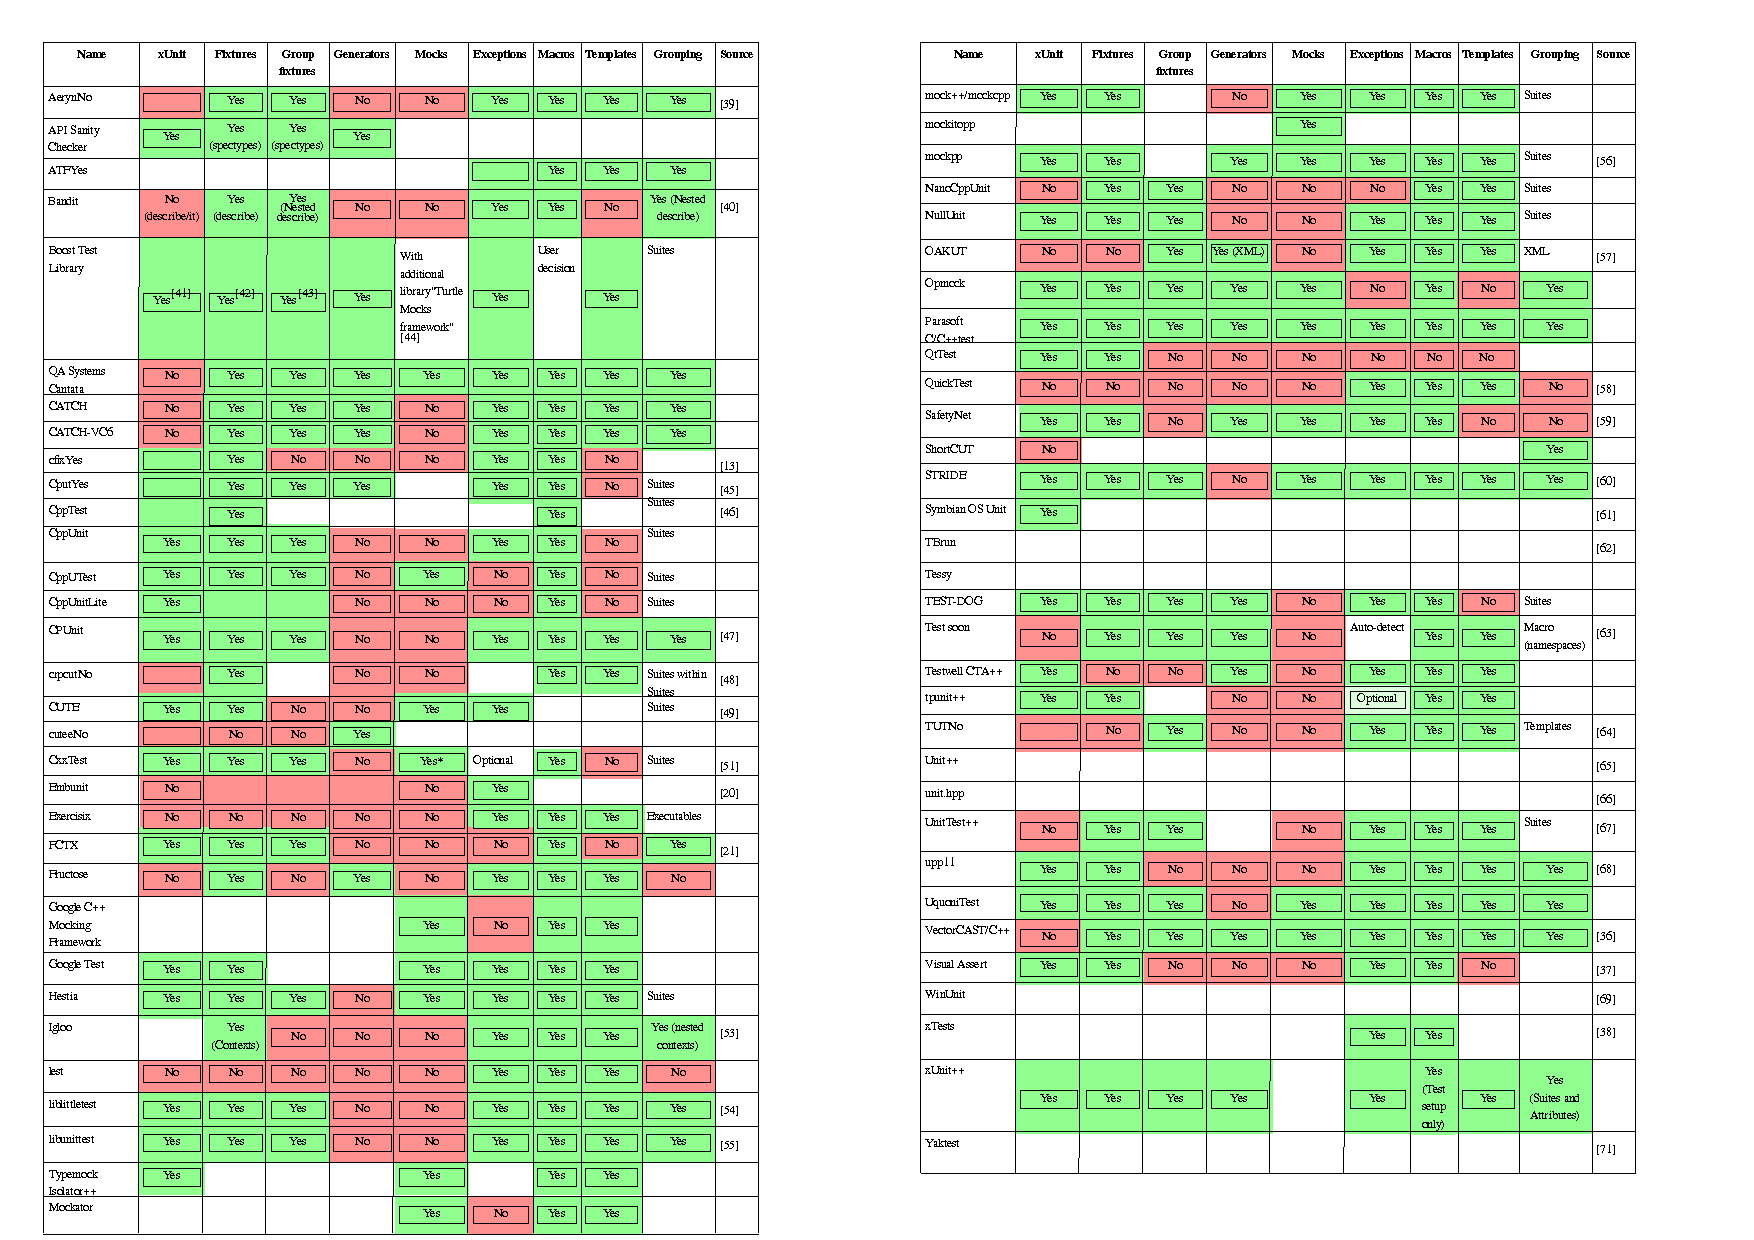
\includegraphics[scale=0.3]{res2/listframeworks_both_1page.pdf}
	\end{center}
	\end{itemize}
\end{frame}

\nextframe
\begin{frame}
	\begin{center}\vspace{70pt}
		{\Huge Thank You All For Listening}\\\vspace{54.35pt}
		GitHub: \url{https://github.com/hartenfels/FSMLplusplus/}
	\end{center}
\end{frame}
\end{document}
